\chapter{Tutorial on setting up time-heterogeneous Epoch Models of substitution in BEAST.\label{app:epoch}}
\chaptermark{Tutorial: Epoch Models of substitution in BEAST}

\section{Introduction}

In this tutorial we will show how to setup, run and analyse data with the epoch models described in \cite{Bielejec2014a}.
We present an artificial example and describe the necessary steps to get an actual analysis up and running.
Example files for this tutorial can be found here \url{http://rega.kuleuven.be/cev/ecv/tutorials/epochExample.zip}.

\section{Prerequisites}

This tutorial assumes that the user has a basic knowledge of the BEAST framework, knows how to generate an XML input file and can interpret basic output information of an MCMC run.
BEAST runnables for all major platforms can be found here \url{http://beast.bio.ed.ac.uk/}.
You will need a Java runtime environment version 1.5 or greater to run the BEAST executable.
Due to the computational intensity of the computations involved in the epoch model, the BEAGLE library also needs to be installed and used with the BEAST runs discussed here.
See \url{https://code.google.com/p/beagle-lib/w/list} for details on how to install and use the BEAGLE library.

\section{Data\label{sec:first}}

Start by uploading your sequences into BEAUTi and generating a standard XML file.
% Sequence file used in this tutorial can be found here \url{URL_GOES_HERE}. 
For simplicity we assume a single nucleotide partition in this example, a constant population size model and a strict molecular clock.

The data in this tutorial was artificially generated by evolving it on an MCC tree generated from a Bayesian phylogenetic analysis of human influenza A hemagglutinin gene sequences sampled through different epidemic seasons \citep{Drummond2010}.
This tree is visualised in Figure~\ref{fig:threeEpoch}.

We will analyze the data with the HKY nucleotide substitution model \citep{hky85}, focusing on estimating the $\kappa$ parameter (i.e., the transition-transversion bias) in three separate epochs.

% FB: Philippe could you work your magic on this figure and mark 3 epochs with transitions at 7 and 15 starting at the tips much like you did for the paper?
\begin{figure}[h!]
\centering
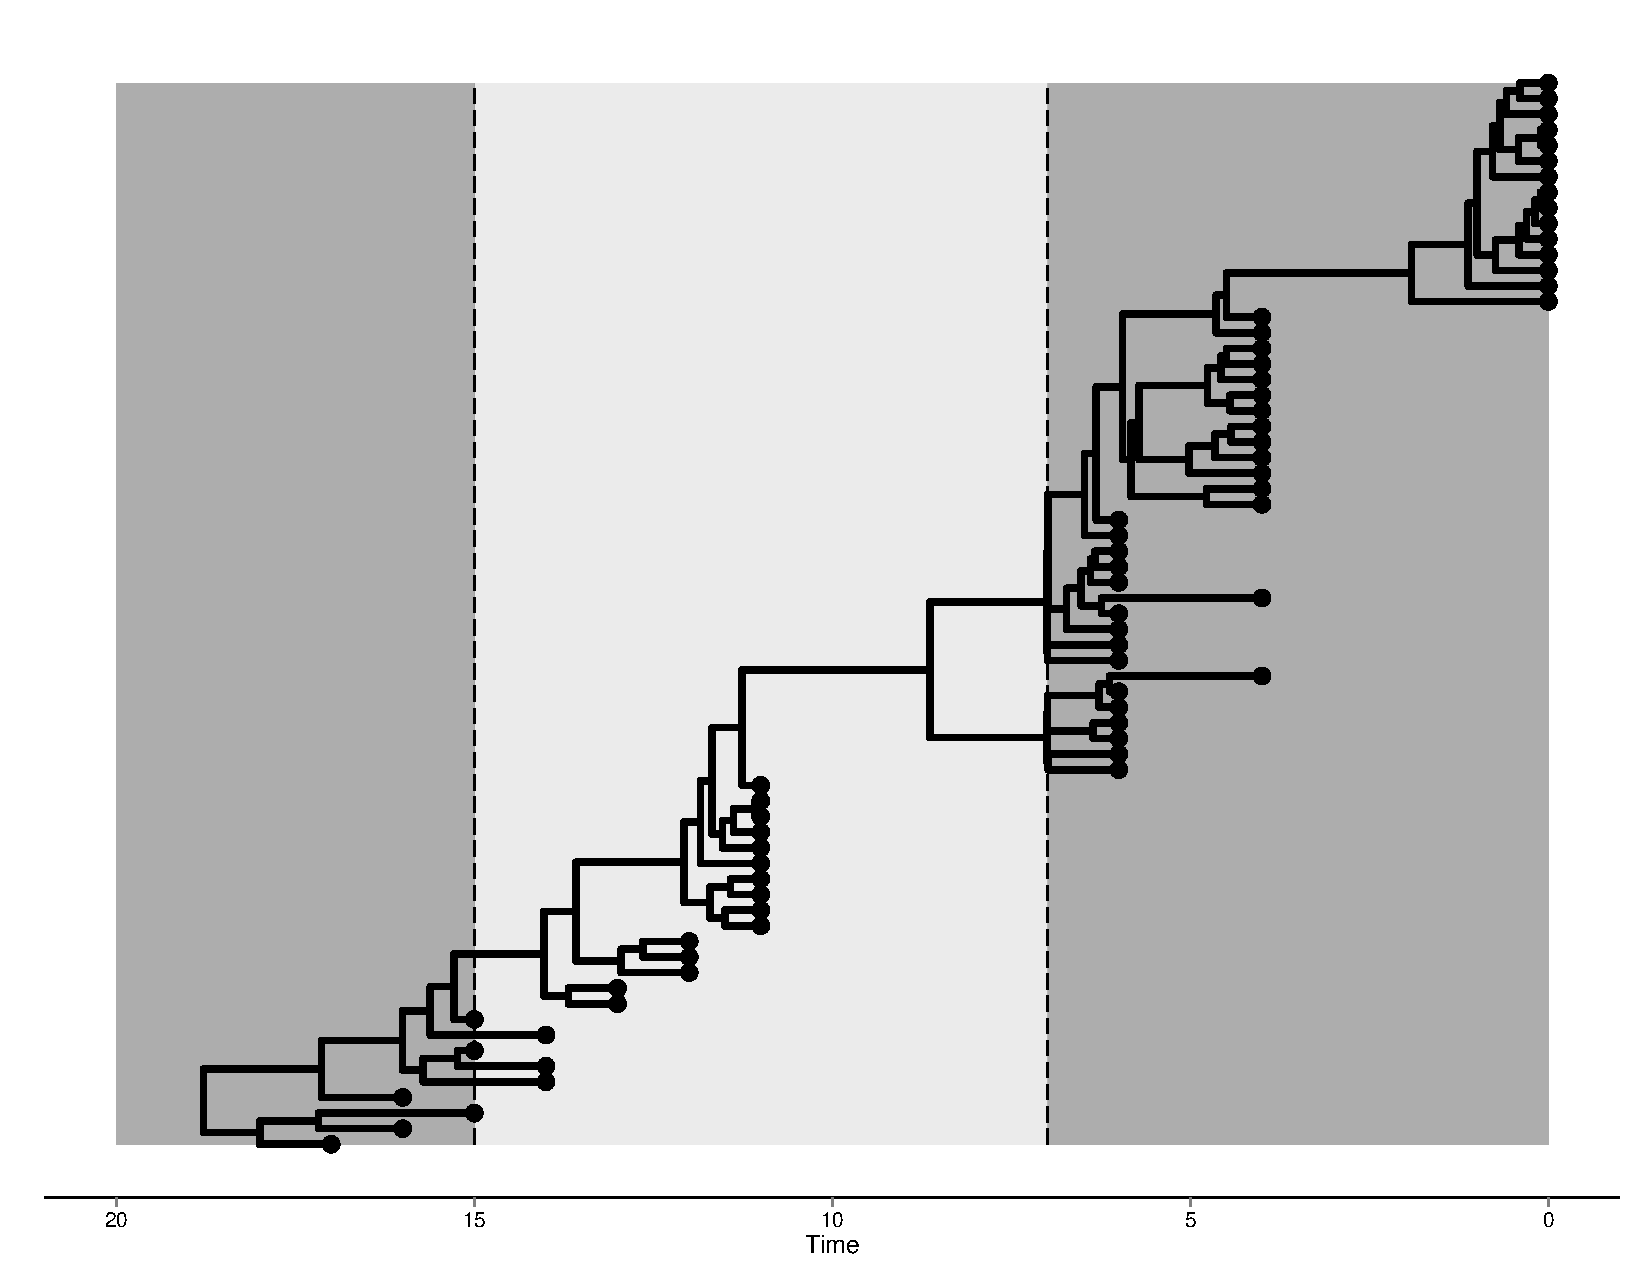
\includegraphics[scale=0.35]{threeEpoch} 
\caption{
{ \footnotesize 
{\bf Tree topology for time-heterogenous analysis.}
} % END: footnotesize
}
\label{fig:threeEpoch}
\end{figure}

The first epoch lasts until transition time $T_{1}$ set at $7$ (7 years before the most recent sampling date) and is governed by a model which we will call \textit{HKY$_1$}.
The second epoch lies between transition times $T_{1}$ and $T_{2}=15$, with substitution model \textit{HKY$_2$}. 
Finally, everything past $T_{2}$ occurs in a third epoch, with corresponding model \textit{HKY$_3$}.



\section{Turning BEAST's XML into an epochized analysis\label{sec:xml}}

Open the file generated in Section~\ref{sec:first} in your favourite text editor.
Scroll down to the block where the HKY model is defined.
We need to define three separate models for each epoch, corresponding to \textit{HKY$_1$}, \textit{HKY$_2$} and \textit{HKY$_3$}, therefore delete this block and paste there: 

% TODO: update references to frequency model
\begin{lstlisting}
  <hkyModel id="hky.1">
    <frequencies>
      <frequencyModel idref="freqModel"/>
    </frequencies>
    <kappa>
      <parameter id="kappa.1" value="1.0" lower="0.0" upper="100.0"/>
    </kappa>
  </hkyModel>

  <hkyModel id="hky.2">
    <frequencies>
      <frequencyModel idref="freqModel"/>
    </frequencies>
    <kappa>
      <parameter id="kappa.2" value="1.0" lower="0.0" upper="100.0"/>
    </kappa>
  </hkyModel>
     
  <hkyModel id="hky.3">
    <frequencies>
      <frequencyModel idref="freqModel"/>
    </frequencies>
    <kappa>
      <parameter id="kappa.3" value="1.0" lower="0.0" upper="100.0"/>
    </kappa>
  </hkyModel>
\end{lstlisting}

The individual models that will make up the epoch model are now available, so we can now setup the epoch model itself.
Below those three blocks paste:

\begin{lstlisting}
  <epochBranchModel id="epochModel">
    <treeModel idref="treeModel"/>

    <epoch id="epoch1" transitionTime="10">
      <hkyModel idref="hky.1"/>
    </epoch>

    <epoch id="epoch2" transitionTime="15">
      <hkyModel idref="hky.2"/>
    </epoch>

    <hkyModel idref="hky.3"/>

  </epochBranchModel>
\end{lstlisting}

Each {\color{darkblue}epoch} block references its corresponding model and transition time that bounds it, with the last (i.e., the furthest in the past) model being unbounded.
Now go to the line in the XML file where the site model is defined.
We need to reference the epoch model we just defined as our substitution model of choice.
Alter the corresponding line to have it look like this:

\begin{lstlisting}
  <siteModel id="siteModel">
    <branchSubstitutionModel> 
      <beagleSubstitutionEpochModel idref="epochModel"/>
    </branchSubstitutionModel> 
  </siteModel>
\end{lstlisting}

Now go to the {\color{darkblue}treeLikelihood} block in the XML file. 
This block also needs to reference the epoch model.
Change the corresponding line to read as follows:

\begin{lstlisting}
  <treeLikelihood id="treeLikelihood">
    <patterns idref="patterns"/>
    <treeModel idref="treeModel"/>
    <siteModel idref="siteModel"/>
    <beagleSubstitutionEpochModel idref="epochModel"/>  
    <strictClockBranchRates idref="branchRates"/>
  </treeLikelihood>
\end{lstlisting}

Since we now have three separate $\kappa$ parameters, we need to define separate transition kernels and separate prior distributions for each of these parameters.
Go to the {\color{darkblue}operators} block. 
Look for an operator which references kappa (our $\kappa$ parameter).
Delete this block and paste there:

\begin{lstlisting}
  <scaleOperator scaleFactor="0.75" weight="0.1">
    <parameter idref="kappa.1"/>
  </scaleOperator>
		
  <scaleOperator scaleFactor="0.75" weight="0.1">
    <parameter idref="kappa.2"/>
  </scaleOperator>
		
  <scaleOperator scaleFactor="0.75" weight="0.1">
    <parameter idref="kappa.3"/>
  </scaleOperator>
\end{lstlisting}

All the other parameters in this analysis are shared, therefore there is no need to define separate transition kernels for them.
Now look for the {\color{darkblue}prior} block, which you can find within the {\color{darkblue}mcmc} block.

We need three prior distributions, one per each $\kappa$ parameter (in this example we assume lognormally distributed $\kappa$ parameters):

% \centering
\begin{lstlisting}
  <logNormalPrior mean="1.0" stdev="2" offset="0.0" meanInRealSpace="true">
    <parameter idref="kappa.1"/>
  </logNormalPrior>
				
  <logNormalPrior mean="1.0" stdev="2" offset="0.0" meanInRealSpace="true">
    <parameter idref="kappa.2"/>
  </logNormalPrior>
				
  <logNormalPrior mean="1.0" stdev="2" offset="0.0" meanInRealSpace="true">
    <parameter idref="kappa.3"/>
  </logNormalPrior>
\end{lstlisting}

Naturally we want to log the three parameters of our epoch model. 
To monitor the analysis we start with the screen log. 
Look for the following line: <{\color{darkblue}log} {\color{darkblue}id}=\textquotedbl{}screenLog \textquotedbl{}{\color{darkblue}logEvery}=\textquotedbl{}5000\textquotedbl{}>.

Find the {\color{darkblue}column} block where the kappa parameter is referenced and paste these three blocks here instead:

\begin{lstlisting}
  <column label="kappa.1" sf="6" width="12">
    <parameter idref="kappa.1"/>
  </column>
			
  <column label="kappa.2" sf="6" width="12">
    <parameter idref="kappa.2"/>
  </column>
			
  <column label="kappa.3" sf="6" width="12">
    <parameter idref="kappa.3"/>
  </column>
\end{lstlisting}

We then still need to modify the lines responsible for storing the parameter estimates of the epoch model to file.
Go to the beginning of the {\color{darkblue}log} block responsible for keeping a log file, i.e. <{\color{darkblue}log} {\color{darkblue}id}=\textquotedbl{}fileLog\textquotedbl{} {\color{darkblue}logEvery}=\textquotedbl{}1000\textquotedbl{}>.
Find the line which references the \textit{kappa} parameter and paste there instead:

\begin{lstlisting}
  <parameter idref="kappa.1"/>
  <parameter idref="kappa.2"/>
  <parameter idref="kappa.3"/>
\end{lstlisting}

We are done with editing the XML and can proceed to performing the analysis.

\section{Running MCMC inference}

Epoch model inference requires the BEAGLE library installed and configured to be visible for BEAST.
Installation and setup of the BEAGLE library on various platforms is covered in \url{https://code.google.com/p/beagle-lib/w/list}.

In a UNIX/Linux environment, the XML edited in section \ref{sec:xml} can be run from the command line using the following command:

\begin{code}
java -Djava.library.path=/usr/local/lib -jar beast.jar epochExample.xml
\end{code}


\section{Analyzing the output}

After the analysis has finished you can import the resulting log file into the software of your choice, e.g. Tracer (a program for analysing the trace files generated by MCMC runs, \url{http://tree.bio.ed.ac.uk/software/tracer/}).

Figure \ref{fig:results} presents the posterior probability distributions of the $\kappa$ parameters, which were our main interest in this analysis. 
%GB: not sure why the line below was needed ...
%Bayesian credibility intervals for all parameter estimates contain the true values of the data.
We can clearly see non-overlapping regions, suggesting that the parameters $\kappa_1$ and $\kappa_3$ are significantly different from the parameter $\kappa_2$.
There is probably no difference between the parameters of the first and the third epoch.

\begin{figure}[h!]
\centering
% Tie Fighter plots!
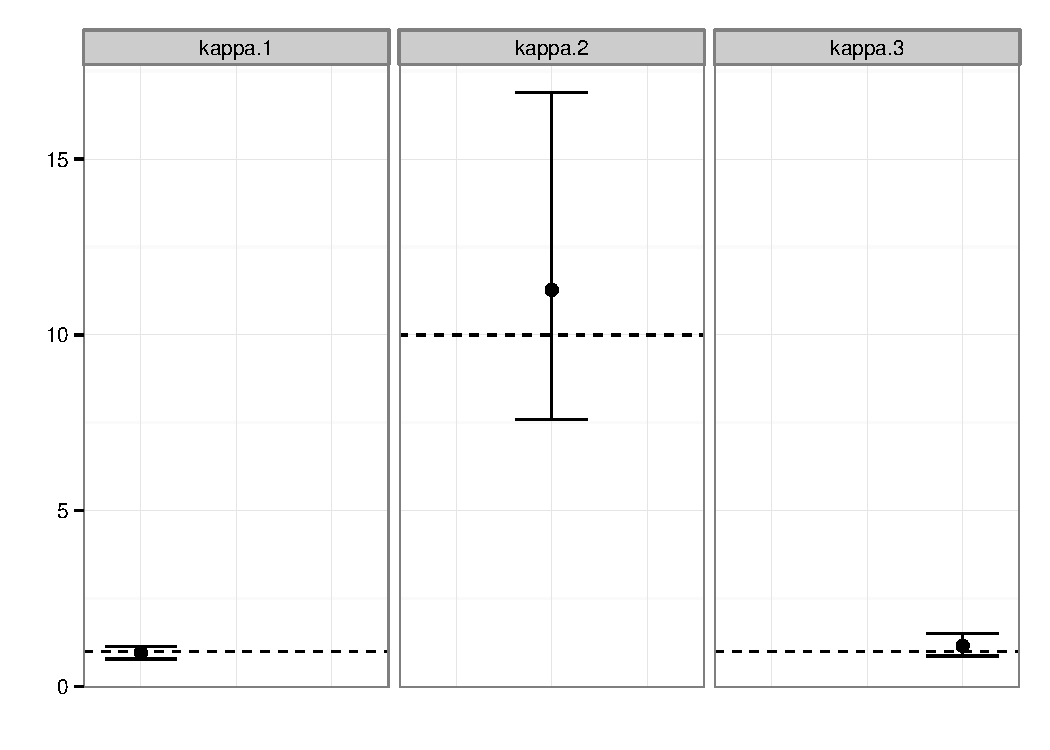
\includegraphics[scale=0.5]{results} 
\caption{
{ \footnotesize 
{\bf 95\% Credible intervals for $\kappa$ parameters.} Horizontal lines mark the true value, black dots indicate posterior mean values.
} % END: footnotesize
}
\label{fig:results}
\end{figure}












% \bibliography{epochtutorefs}
